\section{Theory}
\subsection{Information Segmentation}
\subsubsection{Erosion and Dilation}
\label{subsubsec:Erosion and Dilation}
In our project we need dilation to strengthen small features that we want to be highlighted as well as to get rid of small details in the picture itself. We use it in early preprocessing. It helps together with the erosion to clean up pictures to further process them without too many interfering objects in the image. The main usage is to extract an image that features all the walls and has as few as possible other lines on it \citep{burger_burge_2016}.

For our project we use the binary grayscale erosion.
The erosion uses the following principle to work.


\[A \ominus B = \{ z\in E | B \subseteq A \}\]  
\[where: B_{z} = \{b+z | b \in B\} with \forall z \in E \]

A is a binary image in the Euclidean space or an integer grid. The erosion is done with the structuring element B on the image A. The structuring element has to be a subset or equal to A, otherwise there will be no erosion. The mask B will be applied to all pixels possible, if the mask fits on the center pixel of A, the value will be retained. Otherwise it will get deleted. This means that only when B is completely contained in A, values of pixels are retained.

Binary dilation uses the exact same process. The only difference compared to the erosion is that the deletion of the pixel will not be setting pixel values to white (1) but to black (0). Both of those processes are inherently the same and can be summed up under the term morphological operation. These are altering the image with a mask, as we did here for erosion and dilation.

\subsubsection{Geodesic Dilation}
\label{subsubsec:GeodesicDilation}

Geodesic dilation is an iterative morphological transformation for reconstruction of marked foreground objects. Instead of the normal dilation (Section~\ref{subsubsec:Erosion and Dilation}) it uses a marker image $F$ which defines the starting points of the dilation, a mask image $G$ which defines the constraints of the dilation and a structuring element $B$ which describes the dilation itself.

For example the algorithm is used to reconstruct the area of the brightest points of a distance transformed image (Section~\ref{subsubsec:Distance transformation}). We used this for extracting and enhancing the room center points which then are used as marker points of the watershed marker image (Section~\ref{subsub:watershed}).

The geodesic dilation is defined as $D_{G}^{(n)}(F)$ where n is the iteration size and $F$ the marker with respect to the mask $G$. As a precondition $F$ is a subset of (or is included in) $G$: $F \subseteq G$.

There is no implementation in \gls{gloss:OpenCV} of this algorithm. We implemented it ourself and give here short implementation overview.
	
\begin{equation} \label{eq:geodesic_dilation_iteration}
\begin{gathered}
D_{G}^{(0)}(F) = F
\\
D_{G}^{(1)}(F) = (F \oplus B) \cap G)
\\
D_{G}^{(n)}(F) = D_{G}^{(1)}(D_{G}^{(n-1)}(F))
\end{gathered}
\end{equation}

Where:
\begin{itemize}[label=]
    \item $F$: is the marker image
    \item $G$: is the mask image
    \item $B$: is the structuring element
    \item $n$: is the iteration index
\end{itemize}

As seen in equation~\ref{eq:geodesic_dilation_iteration}, a geodesic dilation with zero iterations is equal to the initial marker image. In the first iteration the marker image $F$ is dilated with the structural element $B$ and the result of that dilation is intersect with the mask image. This intersection limits the dilation to the marker constraints. After one iteration the next iteration uses the result of the last iteration as new marker image $F$.

The iteration stops as soon as the the difference (absolute array norm) between $F^{n}$ and $F^{n-1}$ becomes less then $\epsilon$ which in our case is 0.0001.

\subsubsection{Distance transformation}
\label{subsubsec:Distance transformation}
The distance transformation is as well as the erosion and dilation a morphological operation. In our project it serves the purpose to find bassins for the watershed algorithm. This is used to define the foreground picture. We will explain this further in the wathershed discussion.
It is used after preprocessing to find the center of what is supposed to be rooms. This algorithm is only used in combination with the watershed.

The algorithm that openCV uses is called cvDistTransform and uses an euclidean distance to calculate the output image. The input for this transformation is a binary image \[I(u,v) = I(x)\] which will be separated into a foreground and background image.
\[FG(I) = {x | I(x) = 1}\]
\[BG(I) = {x | I(x) = 0}\]
The formula for the distance transformation of I, D(x) itself is defined as:
\[D(x) :=\min_{x' \in FG(I)} dist(x,x') \]
It applies to any pixel x = (u,v) of the input image. If the pixel is part of the foreground image FG(I) then the result of the transformation D(x) is zero. As said above, the distance formula dist(x,x') is the euclidean distance (also called L\textsubscript{2}-Norm) between two pixels.
\[dist(x,x') = ||x - x'|| = \sqrt{(u - u')^2 + (v - v')^2}\]

Since the exact calculation with the euclidean distance takes a lot of computational power openCV uses the Chamfer-Algorithm instead. This algorithm runs a two masks over the image. The first mask M\textsubscript{L} is run over in a diagonal manner over the image starting in the top left corner of the image. The second mask M\textsubscript{R} does the same in reverse starting at the bottom right corner. Those masks are a matrix that represent the euclidean distance between the center and the pixels around it. Each mask only changes the pixels in the direction they are run through the image \citep{burger_burge_2016}. As a result, the masks look similar to the following ones:
\[M_{L} = \begin{bmatrix} . & . & .\\ . & x & m_1 \\ m_2 & m_1 & m_2 \end{bmatrix}\]
\[M_{R} = \begin{bmatrix} m2 & m1 & m2 \\ m1 & x & . \\ . & . & . \end{bmatrix}\]

This all leads to the resulting effect shown in the image below \citep[Section 3.3.3]{szeliski_2011}.
\todo{Make image of distance transformation before and after}
Source: http://stackoverflow.com/questions/7426136/fastest-available-algorithm-for-distance-transform

\subsubsection{Find contours}
The find-contours algorithm will not receive a detailed description, since it does little more than a simple threshhold in our program. What it is used for is to create the bassins for the watershed algorithm based on the distance transformation. The distance transformation gives us a way to find bassins that are certainly in a room. With the contours-algorithm we create a sharp border for those bassins. Therefore the resulting has a bassin in the center of every room. We can guarantee that this bassin is part of a room and in no way possible part of a wall. In the watershed we will make use of that fact, we will try to connect all bassins to find separate rooms for those that don't connect to others. A more detailed explanation you will find in the watershed section.

\subsubsection{Corner detection}
The corner detection algorithm is used to find corners in an image that contains mostly walls. Its purpose is to find the edges of all walls and therefore provide important information for the door gap closing algorithm. Why this information is needed will be explained in the section about this door gap closing algorithm.
This project uses the harris corner algorithm due to its reliability, simplicity in implementation and the good results we got after the first uses. The algorithm itself is implemented by OpenCv.
The idea of the algorithm is that there are edges wherever the gradient of the image function is high for more than one direction.
First it calculates the basic partial derivatives of the image function I\textsubscript{x}(u,v) in horizontal and vertical direction. This is done for every position in the image (u,v).
\[A(u,v) = I_{x}^2(u,v)\]
\[B(u,v) = I_{y}^2(u,v)\]
\[C(u,v) = I_{x}^2(u,v) * I_{y}^2(u,v)\]

All of those elements will be part of a local structure matrix M.
\[M = \begin{pmatrix} A & C \\ C & B \end{pmatrix}\]
Afterwards all three scalar fields will be smoothed with a linear gaussian filter and be represented as a Matrix \begin{math}\bar{M}\end{math}.
The two eigenvalues of the Matrix \begin{math}\bar{M}\end{math}
\[\lambda_{1,2} = \dfrac{trace(\bar{M})}{2} \pm \sqrt{(\dfrac{trace(\bar{M})}{2})^2 - det(\bar{M})} \]
are positive and contain important information about the local structure. In a area with no corners \begin{math}\bar{M} = 0\end{math}  as well as the two eigenvalues \begin{math}\lambda_1 = \lambda_2 = 0\end{math}. To find a corner there needs to be a strong edge in the main direction (bigger eigenvalue) as well as in the direction of its normal (smaller eigenvalue). 
To find the corner strength itself the harris corner detection uses the function 
\[Q(u,v) := det(\bar{M}(u,v)) - \alpha * (trace(\bar{M}(u,v)))^2\]
whereas the parameter \begin{math}\alpha\end{math} defines the sensitivity of the detector. A candidate for a corner is found when
\[Q(u,v) > t_H\]
with the threshold t\textsubscript{H} being around 10 000 to 1 000 000. To find the exact corner it finds groups of candidates that are close to each other are all eliminated but the best candidate.

\subsubsection{Convex hull}
Finding the convex hull of a set of points is a good way for this project to find the outer points of our wall that is enclosing the whole building. The convex hull is the smallest convex set of points that contains all points given in a Euclidean space.

The convex hull af a set of points X \[conv X \coloneqq \underset{X \subseteq K \subseteq V, K convex}{\bigcap} K  \] is defined as the intersection of all supersets of X.It can also be described as the set of all limited convex combinations:

\[conv X = \{ \sum_{i=1}^{n}\alpha_{i} * x_{i} \mid x_{i} \in X, n \in \mathbb{N}, \sum_{i=1}^{n} \alpha_i = 1, \alpha_i \geq 0  \}]\]

There are several known algorithms that implement this problems. Examples of those are the Graham-Scan algorithm with a complexity of  \[\mathcal{O}(n log n)\] or the Jarvis-March-algorithm with the complexity of \[\mathcal{O}(n*k)\] where k is the number of points on the hull itself.

\begin{figure}[h]
	\centering
	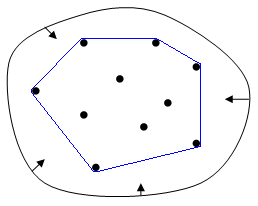
\includegraphics[width=0.4\textwidth]{convex_hull}
	\caption{Example image as to what the convex hull algorithm does.}
	\label{fig:convex_hull}
\end{figure}


\subsubsection{Door gap closing algorithm}

The cascade door training algorithm has found the rectangles that represent the doors. What is needed in the end though is not the door itself but the space inbetween the two walls that the door connects. This is so that we can seperate the different rooms that have doors inbetween.
This algorithm combines the edges that have been found with the Harris-Corner detection and the doors from the cascade door algorithm. It uses a heuristic that works as following. The door algorithm provides four points that mark the edge of the recognized door and build a rectangle.
Added to the rectangle is  a threshold in all directions in which the algorithm searches for edges. The idea is that due to the structure of walls there will be a rectangle made out of four edge points inside the door area that represents the space inbetween the walls. It is expected to only find one rectangle, due to the fact that it makes no sense to have a wall go through a door. As well as the fact that there should be no further lines because it it a cleaned up image and any other line except the walls should not be in that image.
To find the rectangle it connects two edges and calculates the angle compared to the x-Axis for all pairs of edges available. Now all the angles get compared to each other. If two edges AB and CD have a similar angle there will be another comparison for the angles between AC and BD or AD and BC. If one of those two is also of a similar angle we have found our door-rectangle.
\todo{Add image of how those edges are found}

\subsection{Structural Analysis}

\subsubsection{Cascade training}
The algorithm used for object detection in this project was first described by Paul Viola in his paper \todo{ACCEPTED CONFERENCE  ON COMPUTER VISION AND PATTERN RECOGNITION 2001 Rapid Object Detection using a Boosted Cascade of Simple Features}. It is based on three key components. One is the "Integral Image" which is an image representation that allows to detect features very quickly. A second component is the learning algorithm "AdaBoost" which select a small number of critical features from a big set. The last component is an algorithm that combines increasingly complex features in a cascade. All of these components provide the basis for a really fast feature detection compared to previously known algorithms.

The object detection for this method is based on features and not pixels. Features can provide additional domain knowledge that would not be know with just pixels. Additionally the detection based on features is processed much faster than a pixel based system. The algorithm uses three different simple features based on the "Haar" basis functions. The value of a two-rectangle feature is the difference of the sum of two regions that are vertically or horizontally adjacent and have the same measurements (see Figure\todo{link figure}). The three-rectangle feature has the same conditions but the value is based on the sum of two outside rectangles and subtracted the sum of a center rectangle. Last is the four-rectangle features which the value is the difference of sums of diagonal pairs of rectangles.
\begin{figure}[H]
	\centering
	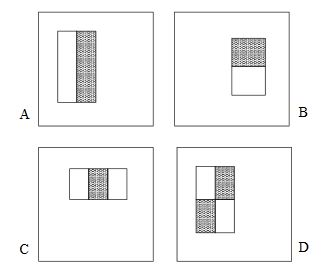
\includegraphics[width=0.4\textwidth]{rectangleFeatures.jpg}
	\caption{Rectangle features in a detection window. There are two-rectangle (A and B), three-rectangle (C) and four-rectangle features in use.}
	\label{fig:rectFeat}
\end{figure}

All features combined are more than 180'000 while the detector has a base resolution of 24x24. This means the rectangle features are overcomplete.
These rectangle features are computed using the representation "integral image". In an integral every pixel is a sum of pixels of the original image that are above and to the left:
\[ii(x,y) = \sum_{x'\leq x, y'\leq y} i(x',y')\]
where ii(x,y) is the integral image and i(x,y) the original. Using two conditions with s(x,y) as the row sum:
\[s(x,y) = s(x,y-1)+i(x,y)\]
\[ii(x,y) = ii(x-1,y)+s(x,y)\]
the whole image can be computed in one pass.
This method helps so we can now compute two-rectangular features from just 6 values instead of having to do all the calculations for the sums each time over whole regions. In addition three-rectangular features only take 8 and four-rectangular only 9 values to calculate its value. This algorithm can only recognize features in vertical, horizontal or diagonal direction due to the nature of our rectangle features.
To train and select a small size of features this algorithm uses the "AdaBoost" method. The basic idea is that there is a feature size over 180'000 features to determine the if an object is recognized or not. The job of this "AdaBoost" is to reduce the amount of features down to a basic set of features that still has a high recognition rate. For each feature the algorithm determines the optimal threshold classification function so that the least amount of examples are misclassified.
To achieve improved detection rate and drastically reduce the computation time this algorithm implements a cascade function. This means that the detection process is that of a degenerate decision tree. A positive result from a classifier triggers the evaluation of the next classifier. If at any point the result is negative the algorithm immediately declares the result as negative and won't be computed any further. The idea is that the first layer rules out a large amount of possibilities with very little computation time. Further stages of the process will reduce further negatives but need additional computation power. The idea behind this process is that in an image most sub-windows will be negative and such should be rejected as early as possible in the cascade process to require fewer computational effort.
The classifier is trained with a training set of positives and negatives. Each stage is trained by adding features until the target detection and false positive rates are met. Stages are added until the overall target for false positive rate and detection rate is met. In the end there is always a balance to between finding high detection rates with low false positive rates and lower time for computation.

 
\subsection{Semantic Analysis}
\subsubsection{Hough transformation}
\label{subsubsec:Hough transformation}
The hough transformation was used as an alternative to the current process to find walls and therefore the rooms. In the implementation it will be explained why this was not implemented in the final project.

What the hough transformation does is to find 

\todo{finish this chapter!}

\pagebreak

\subsubsection{Connected Component Analysis}
Finding connected components is a common way to detect objects in a thresholded image. In this work it is used to detect connected room pixels and calculate the size of each room out of it.

This is accomplished by finding pixels which are adjacent to each other. A pixel is adjacent to another pixel if it is immediate $\mathcal{N}_4$ or $\mathcal{N}_8$ and has the same scalar value. Further the neighbour pixels are labeled with the same label and in the end combined to a region $\mathcal{R}$ \citep[Section 3.3.4]{szeliski_2011}.

\begin{figure}[h]
	\centering
	\subfloat[4-neighbourhood, $\mathcal{N}_4$]{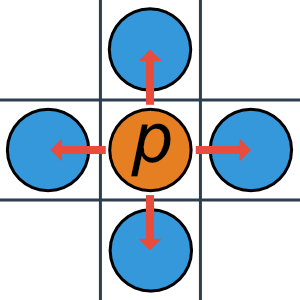
\includegraphics[width=0.3\textwidth]{n4_pixel}\label{fig:n4_pixel}}
	\hfill
	\subfloat[8-neighbourhood, $\mathcal{N}_8$]{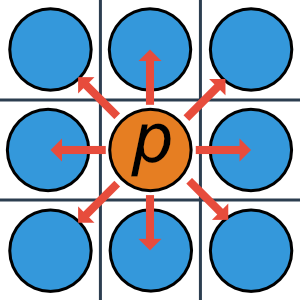
\includegraphics[width=0.3\textwidth]{n8_pixel}\label{fig:n8_pixel}}
	\caption{Pixel neighbourhoods.}
	\label{fig:pixel_neighbourhood}
\end{figure}

The distance $\mathcal{N}_4$ and $\mathcal{N}_8$ refers to the distance between two pixels (Figure~\ref{fig:pixel_neighbourhood}). In $\mathcal{N}_4$ only the four pixels (top, left, bottom, right) are used to determine if two pixels are connected. In $\mathcal{N}_8$ all pixels around the pixel are included into the process \citep{burger_burge_2016}.

For each region $\mathcal{R}$ it is possible to compute statistics like the area (number of pixels) or the perimeter (number of boundary pixels) \citep[Section 3.3.4]{szeliski_2011}. These statistics are used for example to determine the actual room size.

\subsubsection{Watershed}
\label{subsub:watershed}
The watershed-algorithm in our project is used for segmentation of the different rooms. It can find rooms indifferent of its shape.
\\
The algorithm is processed on a grayscale image on which the color intensity is analogous to the height in a height map. The watershed in use does flooding. The idea is to place a water source in each regional minimum and flood the entire relief. It will stop if it meets a different watersource or an impassable barrier.

The basic algorithm uses three different markings for all regions. The values I for each region can be:
\[I(u,v) = \begin{cases} 0 & background \\  255 & foreground \\ 1..254 & regions \end{cases} \]

It is a really simple algorithm where it starts with looking for an unmarked foreground pixel. All pixels of the region that are connected to this starting pixel will be visited and marked. There are three different ways to do this process. It can be a recursive, an iterative depth-first or breadth-first flood filling. It is not clear what implementation OpenCv uses. In the end all of the methods lead to a similar result and thus will not be discussed further. 

